\section{Cracking Pattern caused by Pure ASR Expansion}

\subsection{ASR Expansion Simulation of Single Aggregate Case}

In this section, simulation of ASR expansion on a single aggregate case in size only $10 \times 10 \times 10$ mm is presented(Figure \ref{smallasr}).

Since this model is very small and simple, it is easier to analyze the behavior of ASR expansion in very small scale around coarse aggregate.

The expanse is generated at the location of interfaces between mortar and aggregate, to introduce the expansion, as introduced in chapter 2.

%TODO: Single Aggregate 3D, 2D

\begin{figure}[h!]
\centering
%*******
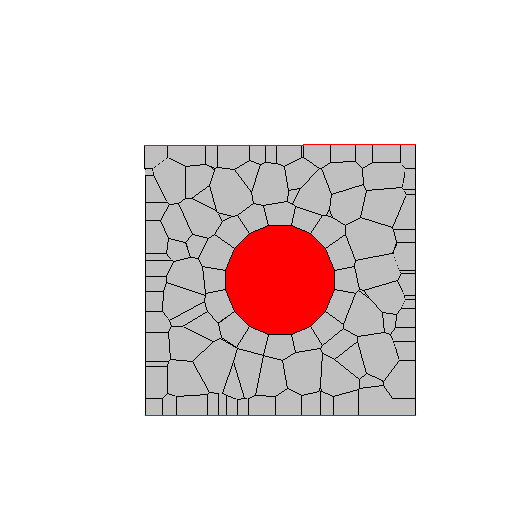
\includegraphics[width=0.4\linewidth]{Files/Small_ASR/CR/DEP5-STEP(001).png}
\caption{Single Aggregate Case in Size $10 \times 10 \times 10$ mm}
\label{smallasr}
\end{figure}

0.001 initial strain is introduced in each step at the interfaces between the aggregate and paste elements. Totally 20 steps of expansion are done.

% Small ASR CR
  \begin{figure}[ht!]
  \centering
      %*******
      \begin{subfigure}{.25\textwidth}
        \centering
        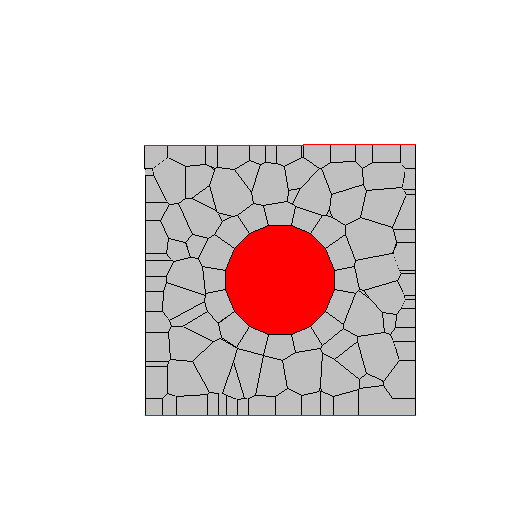
\includegraphics[width=1.0\linewidth]{Files/Small_ASR/CR/DEP5-STEP(001).png}
      \caption{Step 1}
      \end{subfigure}%
      %*******
      \begin{subfigure}{.25\textwidth}
        \centering
        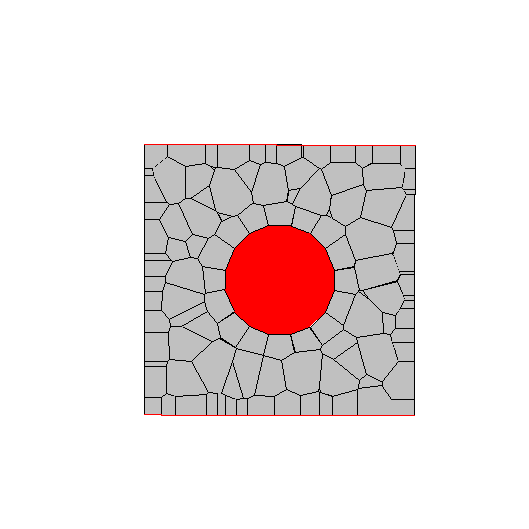
\includegraphics[width=1.0\linewidth]{Files/Small_ASR/CR/DEP5-STEP(002).png}
      \caption{Step 2}
      \end{subfigure}%
      %*******
      \begin{subfigure}{.25\textwidth}
        \centering
        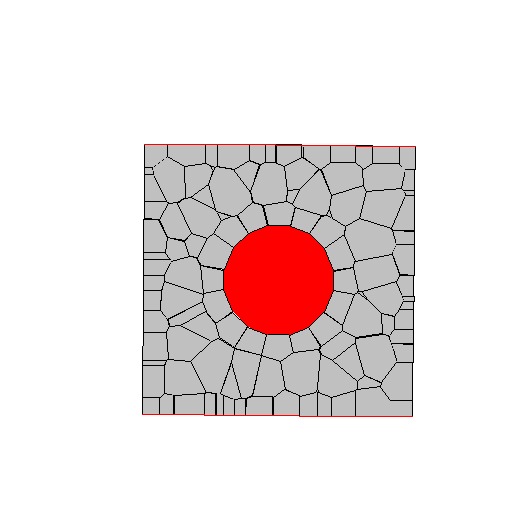
\includegraphics[width=1.0\linewidth]{Files/Small_ASR/CR/DEP5-STEP(003).png}
      \caption{Step 3}
      \end{subfigure}%
      %*******
      \begin{subfigure}{.25\textwidth}
        \centering
        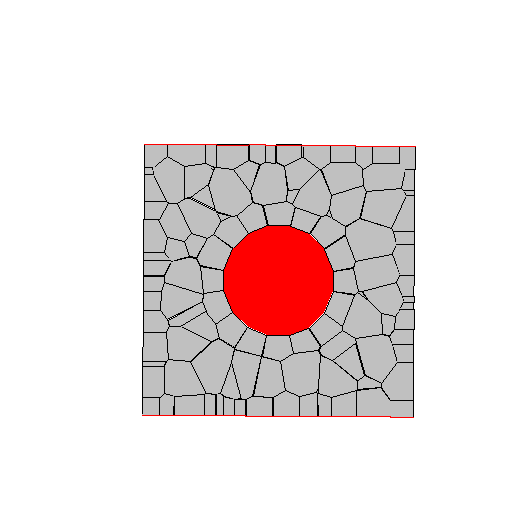
\includegraphics[width=1.0\linewidth]{Files/Small_ASR/CR/DEP5-STEP(004).png}
      \caption{Step 4}
      \end{subfigure}

      %*******
      %*******
      \begin{subfigure}{.25\textwidth}
        \centering
        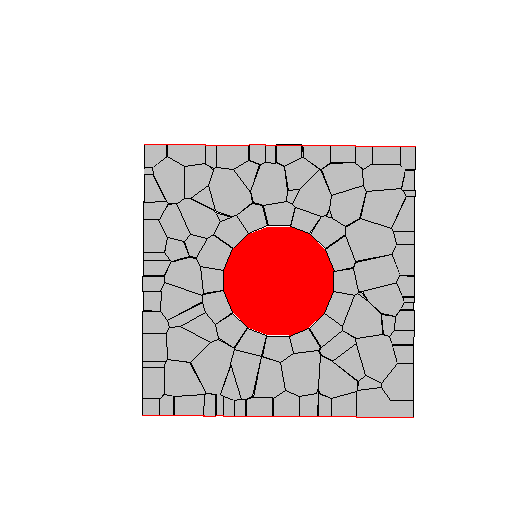
\includegraphics[width=1.0\linewidth]{Files/Small_ASR/CR/DEP5-STEP(005).png}
      \caption{Step 5}
      \end{subfigure}%
      %*******
      \begin{subfigure}{.25\textwidth}
        \centering
        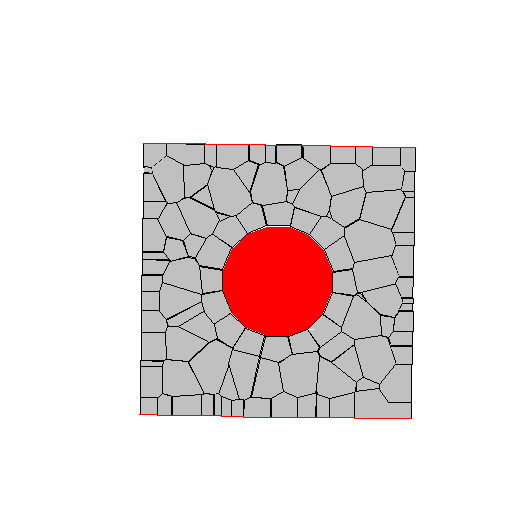
\includegraphics[width=1.0\linewidth]{Files/Small_ASR/CR/DEP5-STEP(006).png}
      \caption{Step 6}
      \end{subfigure}%
      %*******
      \begin{subfigure}{.25\textwidth}
        \centering
        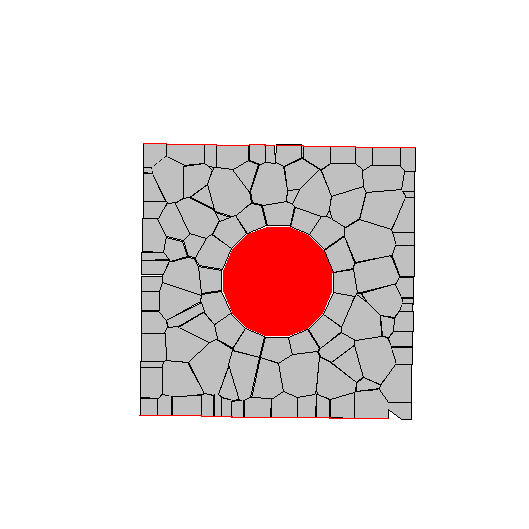
\includegraphics[width=1.0\linewidth]{Files/Small_ASR/CR/DEP5-STEP(007).png}
      \caption{Step 7}
      \end{subfigure}%
      %*******
      \begin{subfigure}{.25\textwidth}
        \centering
        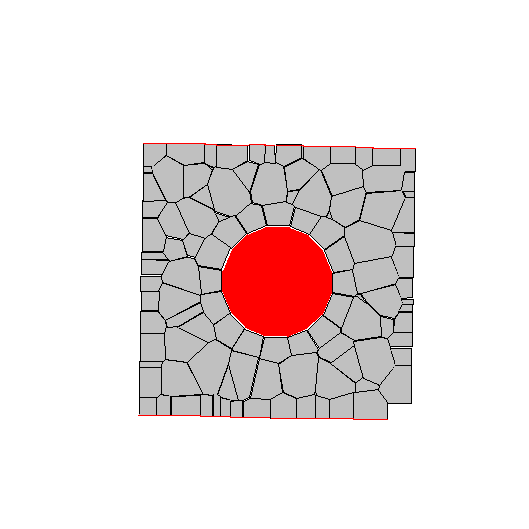
\includegraphics[width=1.0\linewidth]{Files/Small_ASR/CR/DEP5-STEP(008).png}
      \caption{Step 4}
      \end{subfigure}

      %*******
      %*******
      \begin{subfigure}{.25\textwidth}
        \centering
        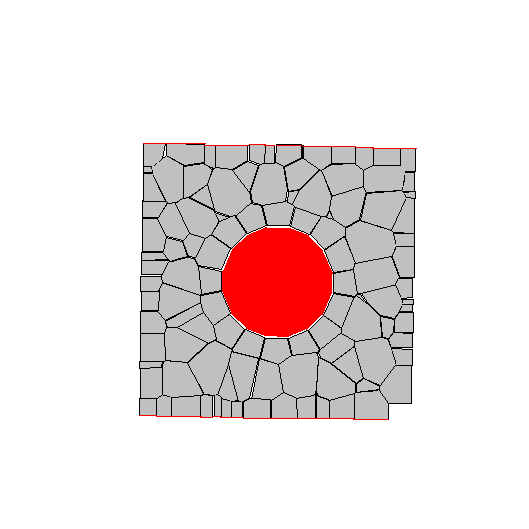
\includegraphics[width=1.0\linewidth]{Files/Small_ASR/CR/DEP5-STEP(009).png}
      \caption{Step 9}
      \end{subfigure}%
      %*******
      \begin{subfigure}{.25\textwidth}
        \centering
        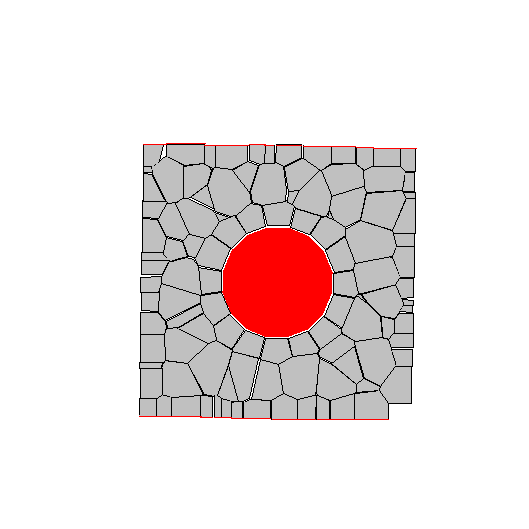
\includegraphics[width=1.0\linewidth]{Files/Small_ASR/CR/DEP5-STEP(010).png}
      \caption{Step 10}
      \end{subfigure}%
      %*******
      \begin{subfigure}{.25\textwidth}
        \centering
        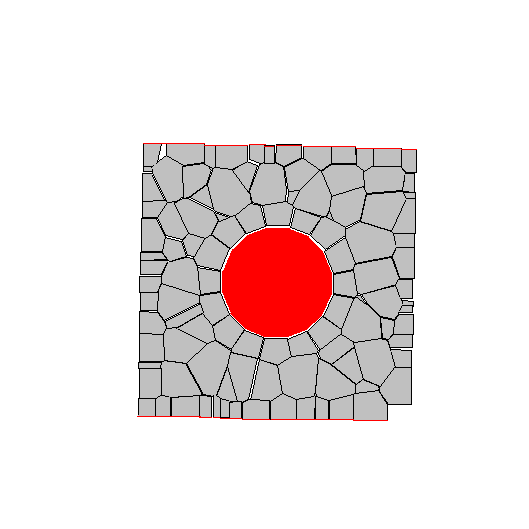
\includegraphics[width=1.0\linewidth]{Files/Small_ASR/CR/DEP5-STEP(011).png}
      \caption{Step 11}
      \end{subfigure}%
      %*******
      \begin{subfigure}{.25\textwidth}
        \centering
        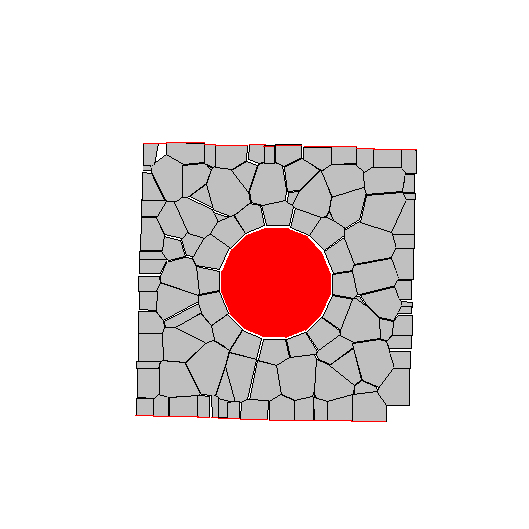
\includegraphics[width=1.0\linewidth]{Files/Small_ASR/CR/DEP5-STEP(012).png}
      \caption{Step 12}
      \end{subfigure}

      %*******
      %*******
      \begin{subfigure}{.25\textwidth}
        \centering
        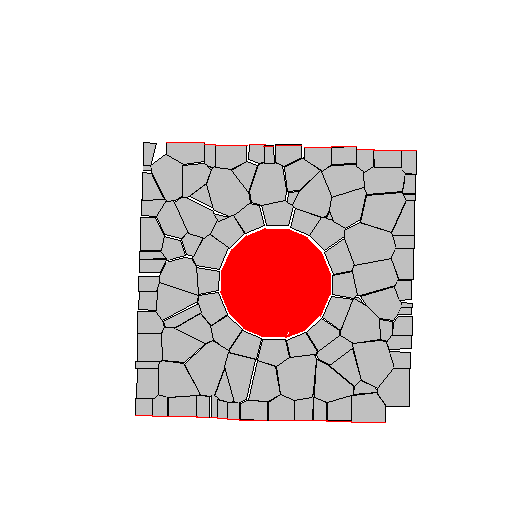
\includegraphics[width=1.0\linewidth]{Files/Small_ASR/CR/DEP5-STEP(013).png}
      \caption{Step 13}
      \end{subfigure}%
      %*******
      \begin{subfigure}{.25\textwidth}
        \centering
        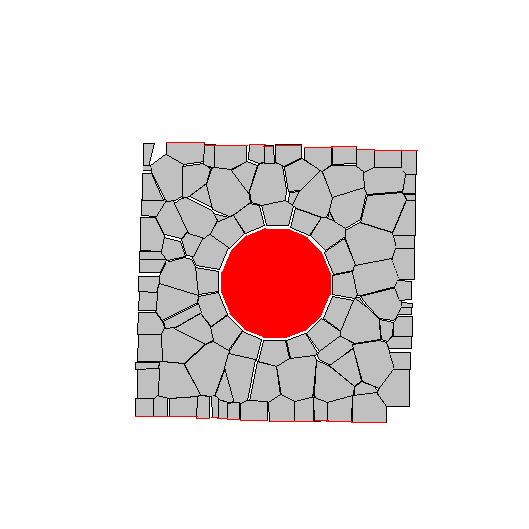
\includegraphics[width=1.0\linewidth]{Files/Small_ASR/CR/DEP5-STEP(014).png}
      \caption{Step 14}
      \end{subfigure}%
      %*******
      \begin{subfigure}{.25\textwidth}
        \centering
        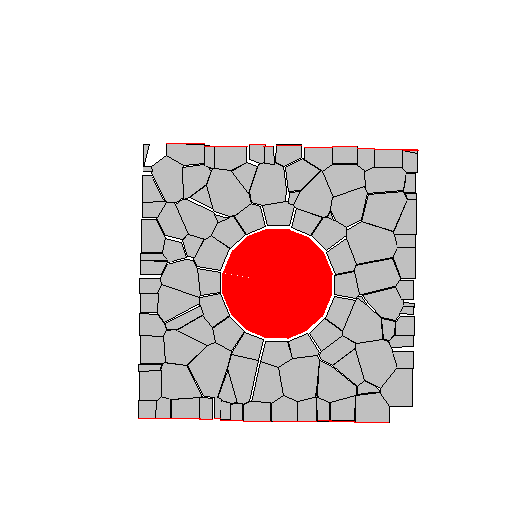
\includegraphics[width=1.0\linewidth]{Files/Small_ASR/CR/DEP5-STEP(015).png}
      \caption{Step 15}
      \end{subfigure}%
      %*******
      \begin{subfigure}{.25\textwidth}
        \centering
        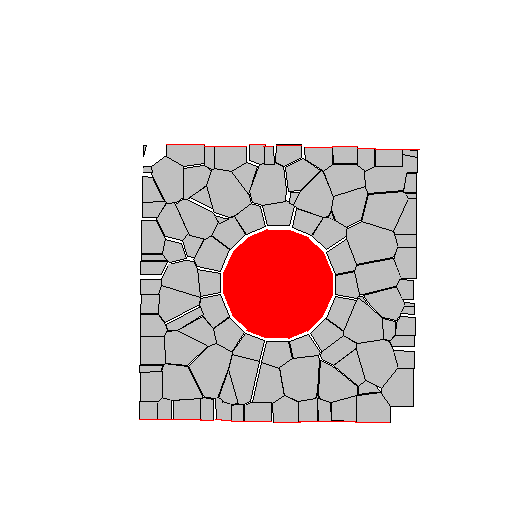
\includegraphics[width=1.0\linewidth]{Files/Small_ASR/CR/DEP5-STEP(016).png}
      \caption{Step 16}
      \end{subfigure}

      %*******
      %*******
      \begin{subfigure}{.25\textwidth}
        \centering
        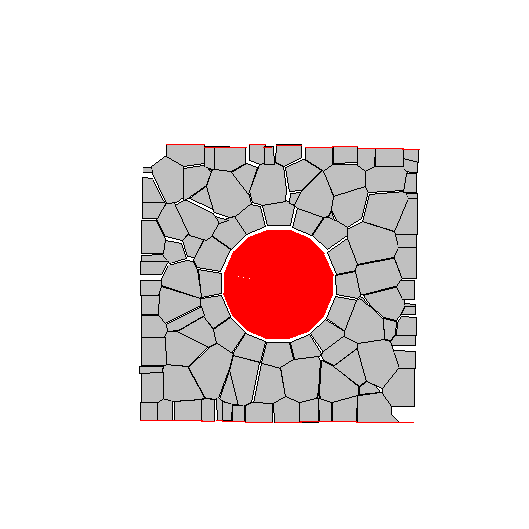
\includegraphics[width=1.0\linewidth]{Files/Small_ASR/CR/DEP5-STEP(017).png}
      \caption{Step 17}
      \end{subfigure}%
      %*******
      \begin{subfigure}{.25\textwidth}
        \centering
        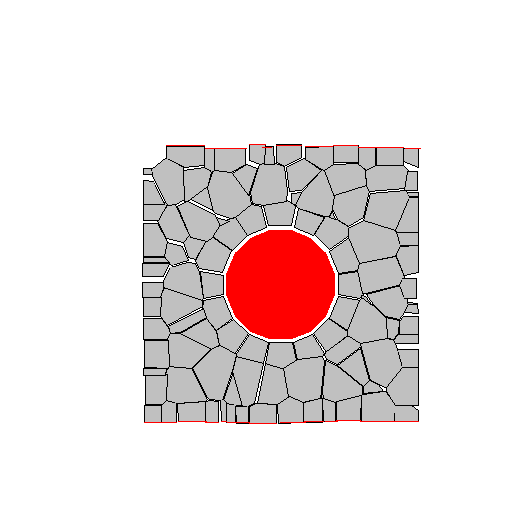
\includegraphics[width=1.0\linewidth]{Files/Small_ASR/CR/DEP5-STEP(018).png}
      \caption{Step 18}
      \end{subfigure}%
      %*******
      \begin{subfigure}{.25\textwidth}
        \centering
        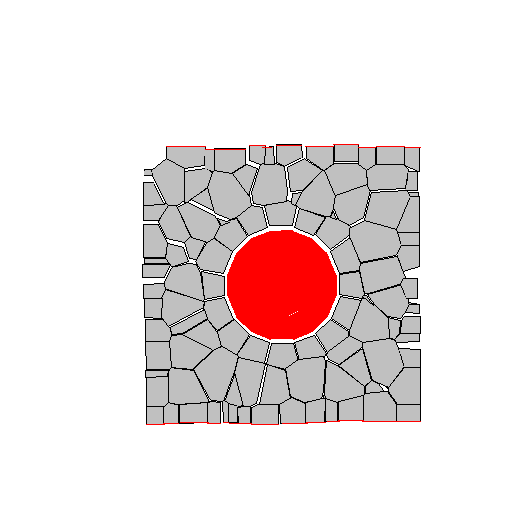
\includegraphics[width=1.0\linewidth]{Files/Small_ASR/CR/DEP5-STEP(019).png}
      \caption{Step 19}
      \end{subfigure}%
      %*******
      \begin{subfigure}{.25\textwidth}
        \centering
        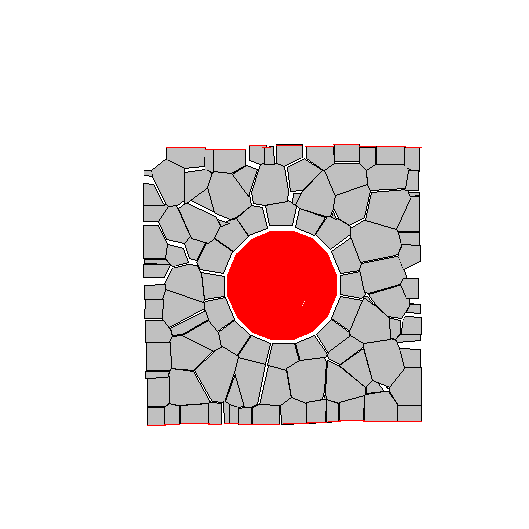
\includegraphics[width=1.0\linewidth]{Files/Small_ASR/CR/DEP5-STEP(020).png}
      \caption{Step 20}
      \end{subfigure}

      \begin{subfigure}{0.8\textwidth}
  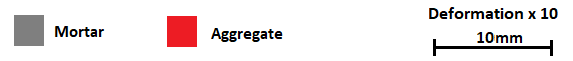
\includegraphics[width=0.8\linewidth]{Files/exp_3D/tag_crack_s.png}
\end{subfigure}%


  \caption{Cross Section in Each Step for ASR $10 \times 10 \times 10$ mm Case ($Deformation \times 10$)}
  \label{fig:ASR_Small_ASR_CR}
  \end{figure}


From the Figure \ref{fig:ASR_Small_ASR_CR}, we can see that step by step with initial stain introducing into the model, distance appears between aggregate and the surrounding element at first, which theoretically should be filled by ASR gel, the product of ASR reaction.

After, by the influence of the unbalanced force start from the aggregate-mortar interfaces, elements surround it also react. Cracks start to generate from aggregate to the paste surrounding it.

The total volume of this small model is increasing step by step, while until the step 20 the model expanded 0.1625\% one dimensionally.

% Small ASR IS
  \begin{figure}[ht!]
  \centering
      %*******
      \begin{subfigure}{.25\textwidth}
        \centering
        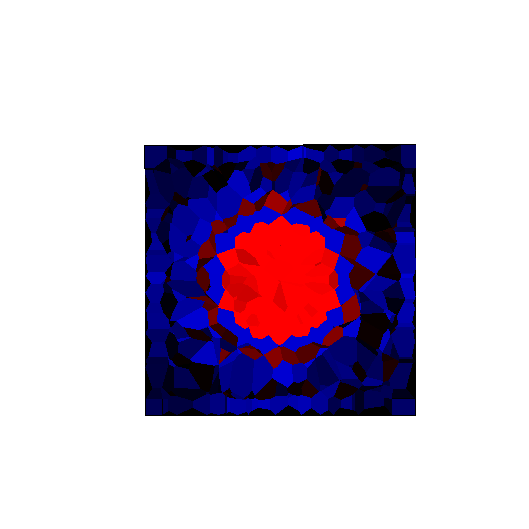
\includegraphics[width=1.0\linewidth]{Files/Small_ASR/IS/DEP5-STEP(001).png}
      \caption{Step 1}
      \end{subfigure}%
      %*******
      \begin{subfigure}{.25\textwidth}
        \centering
        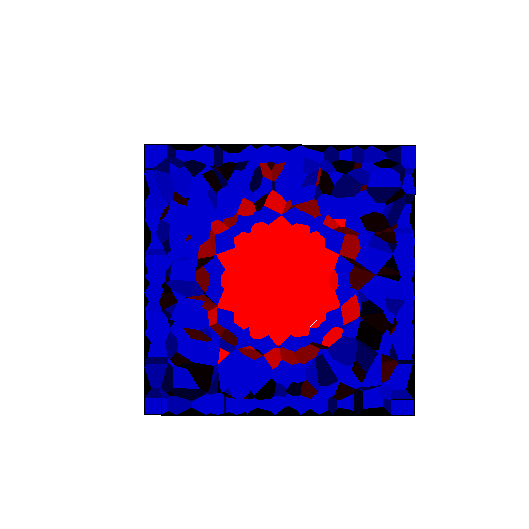
\includegraphics[width=1.0\linewidth]{Files/Small_ASR/IS/DEP5-STEP(002).png}
      \caption{Step 2}
      \end{subfigure}%
      %*******
      \begin{subfigure}{.25\textwidth}
        \centering
        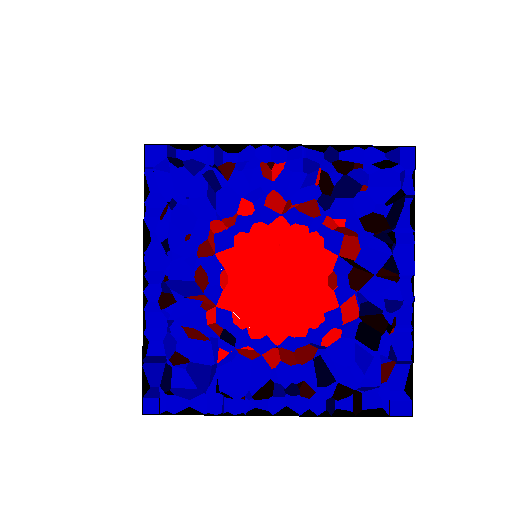
\includegraphics[width=1.0\linewidth]{Files/Small_ASR/IS/DEP5-STEP(003).png}
      \caption{Step 3}
      \end{subfigure}%
      %*******
      \begin{subfigure}{.25\textwidth}
        \centering
        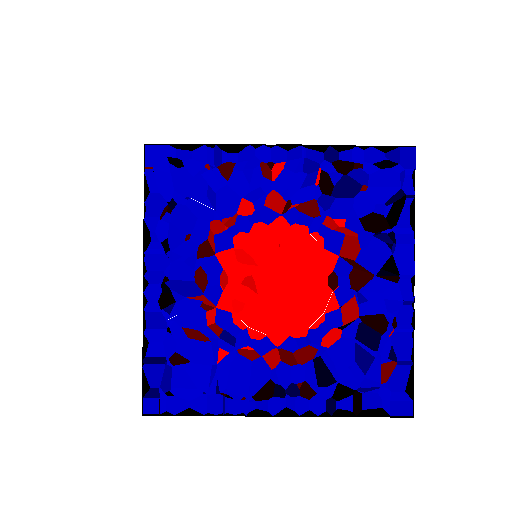
\includegraphics[width=1.0\linewidth]{Files/Small_ASR/IS/DEP5-STEP(004).png}
      \caption{Step 4}
      \end{subfigure}

      %*******
      %*******
      \begin{subfigure}{.25\textwidth}
        \centering
        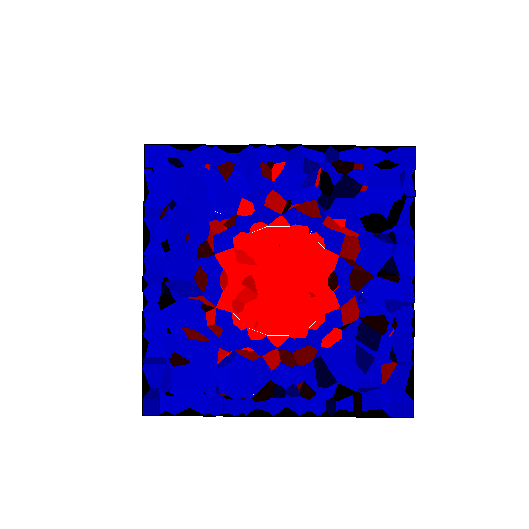
\includegraphics[width=1.0\linewidth]{Files/Small_ASR/IS/DEP5-STEP(005).png}
      \caption{Step 5}
      \end{subfigure}%
      %*******
      \begin{subfigure}{.25\textwidth}
        \centering
        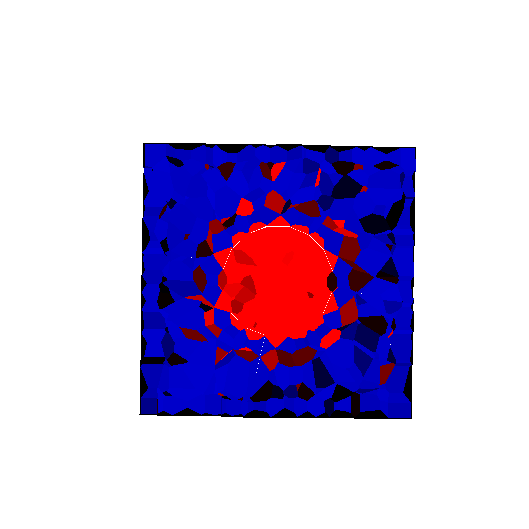
\includegraphics[width=1.0\linewidth]{Files/Small_ASR/IS/DEP5-STEP(006).png}
      \caption{Step 6}
      \end{subfigure}%
      %*******
      \begin{subfigure}{.25\textwidth}
        \centering
        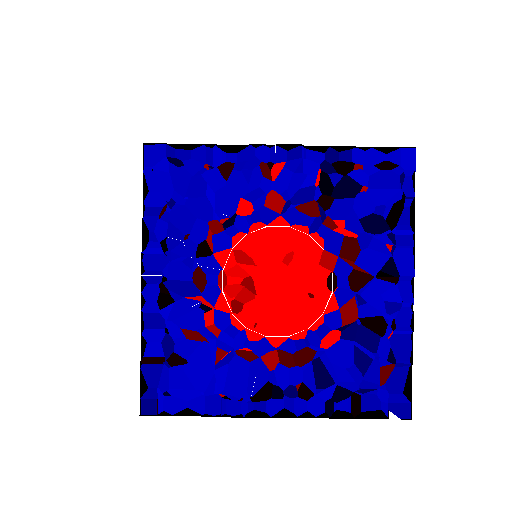
\includegraphics[width=1.0\linewidth]{Files/Small_ASR/IS/DEP5-STEP(007).png}
      \caption{Step 7}
      \end{subfigure}%
      %*******
      \begin{subfigure}{.25\textwidth}
        \centering
        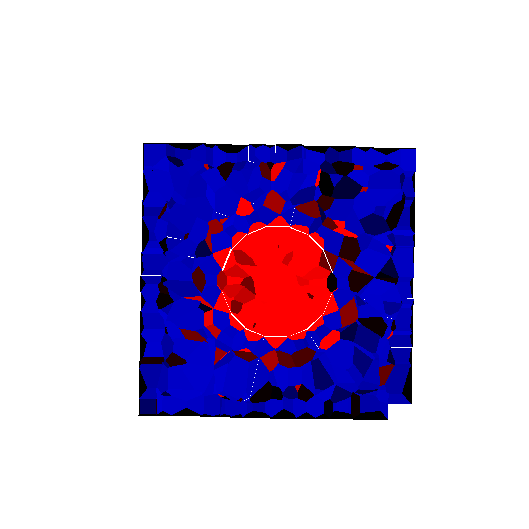
\includegraphics[width=1.0\linewidth]{Files/Small_ASR/IS/DEP5-STEP(008).png}
      \caption{Step 4}
      \end{subfigure}

      %*******
      %*******
      \begin{subfigure}{.25\textwidth}
        \centering
        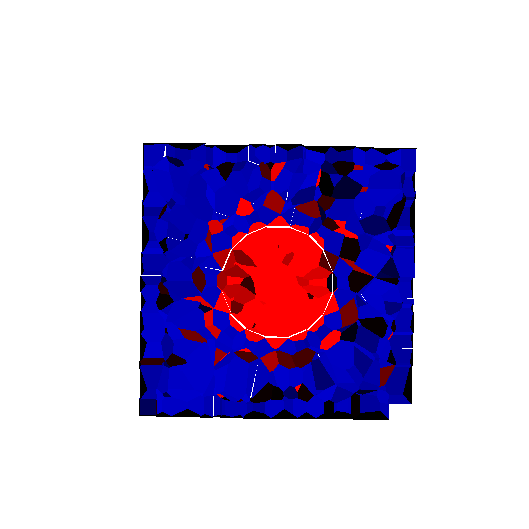
\includegraphics[width=1.0\linewidth]{Files/Small_ASR/IS/DEP5-STEP(009).png}
      \caption{Step 9}
      \end{subfigure}%
      %*******
      \begin{subfigure}{.25\textwidth}
        \centering
        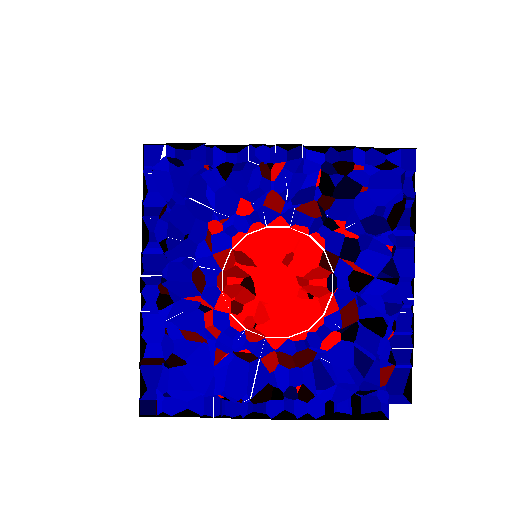
\includegraphics[width=1.0\linewidth]{Files/Small_ASR/IS/DEP5-STEP(010).png}
      \caption{Step 10}
      \end{subfigure}%
      %*******
      \begin{subfigure}{.25\textwidth}
        \centering
        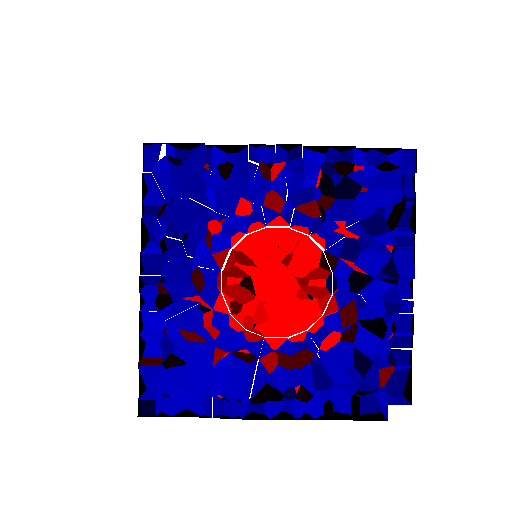
\includegraphics[width=1.0\linewidth]{Files/Small_ASR/IS/DEP5-STEP(011).png}
      \caption{Step 11}
      \end{subfigure}%
      %*******
      \begin{subfigure}{.25\textwidth}
        \centering
        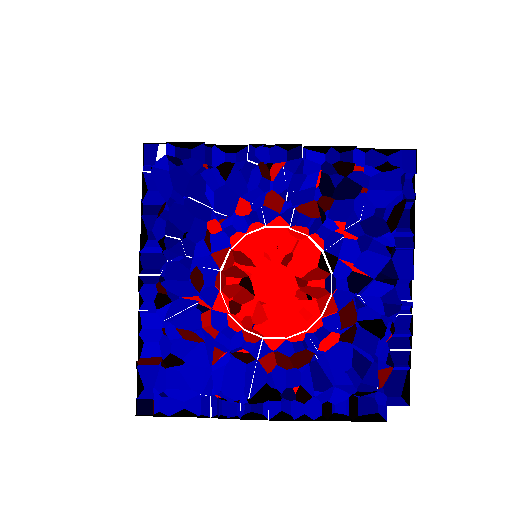
\includegraphics[width=1.0\linewidth]{Files/Small_ASR/IS/DEP5-STEP(012).png}
      \caption{Step 12}
      \end{subfigure}

      %*******
      %*******
      \begin{subfigure}{.25\textwidth}
        \centering
        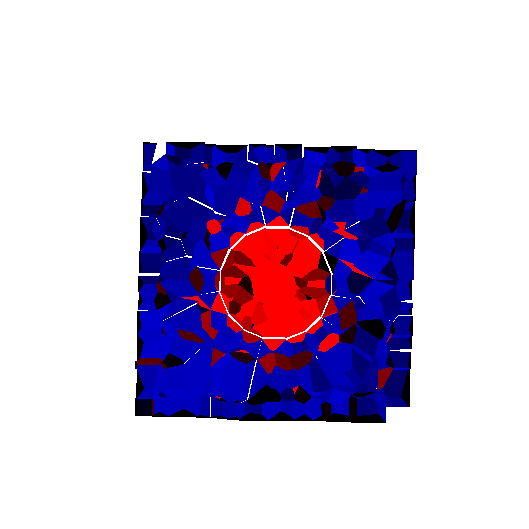
\includegraphics[width=1.0\linewidth]{Files/Small_ASR/IS/DEP5-STEP(013).png}
      \caption{Step 13}
      \end{subfigure}%
      %*******
      \begin{subfigure}{.25\textwidth}
        \centering
        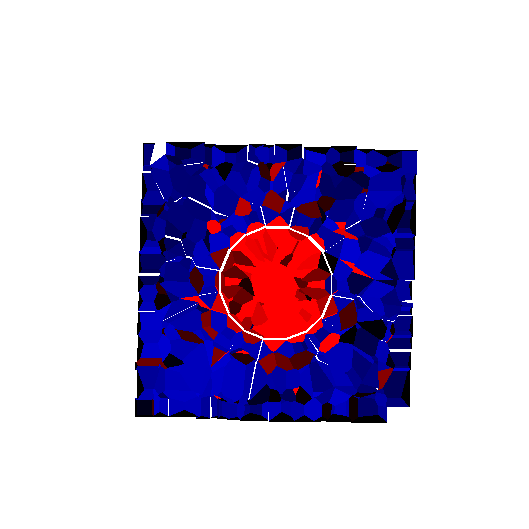
\includegraphics[width=1.0\linewidth]{Files/Small_ASR/IS/DEP5-STEP(014).png}
      \caption{Step 14}
      \end{subfigure}%
      %*******
      \begin{subfigure}{.25\textwidth}
        \centering
        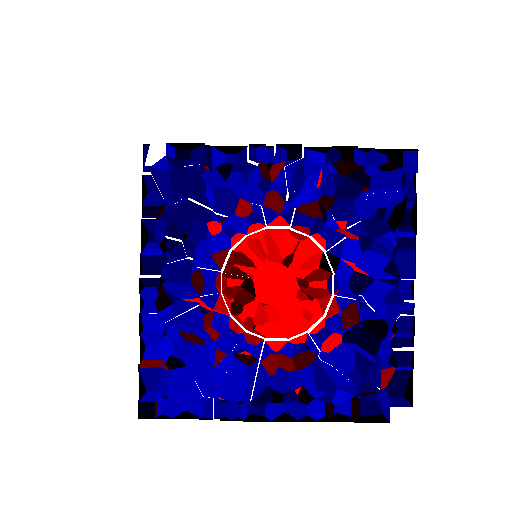
\includegraphics[width=1.0\linewidth]{Files/Small_ASR/IS/DEP5-STEP(015).png}
      \caption{Step 15}
      \end{subfigure}%
      %*******
      \begin{subfigure}{.25\textwidth}
        \centering
        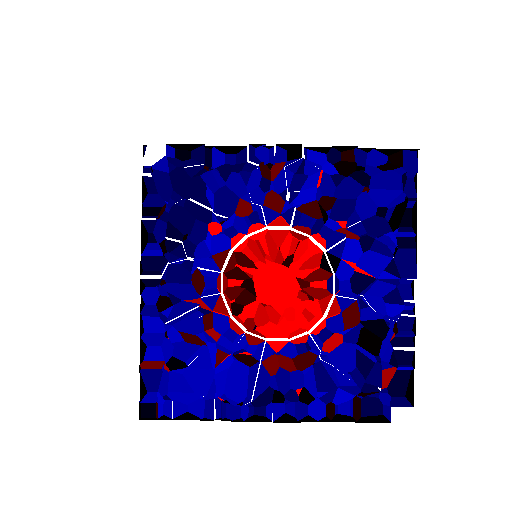
\includegraphics[width=1.0\linewidth]{Files/Small_ASR/IS/DEP5-STEP(016).png}
      \caption{Step 16}
      \end{subfigure}

      %*******
      %*******
      \begin{subfigure}{.25\textwidth}
        \centering
        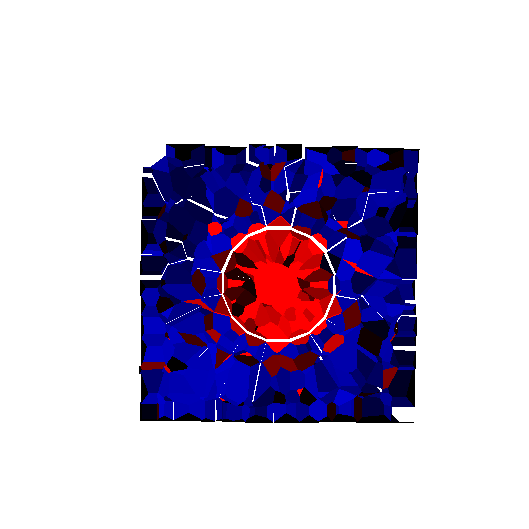
\includegraphics[width=1.0\linewidth]{Files/Small_ASR/IS/DEP5-STEP(017).png}
      \caption{Step 17}
      \end{subfigure}%
      %*******
      \begin{subfigure}{.25\textwidth}
        \centering
        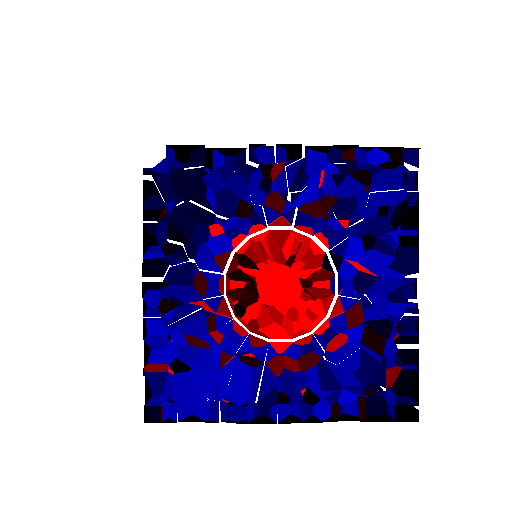
\includegraphics[width=1.0\linewidth]{Files/Small_ASR/IS/DEP5-STEP(018).png}
      \caption{Step 18}
      \end{subfigure}%
      %*******
      \begin{subfigure}{.25\textwidth}
        \centering
        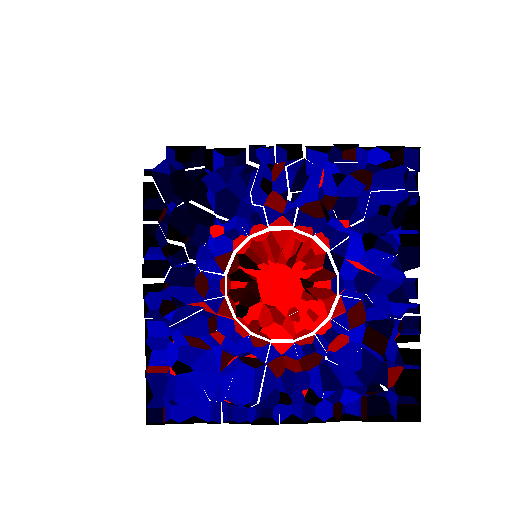
\includegraphics[width=1.0\linewidth]{Files/Small_ASR/IS/DEP5-STEP(019).png}
      \caption{Step 19}
      \end{subfigure}%
      %*******
      \begin{subfigure}{.25\textwidth}
        \centering
        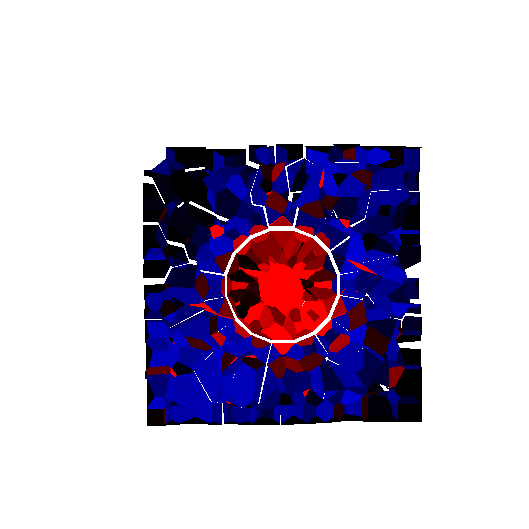
\includegraphics[width=1.0\linewidth]{Files/Small_ASR/IS/DEP5-STEP(020).png}
      \caption{Step 20}
      \end{subfigure}

      \begin{subfigure}{0.8\textwidth}
  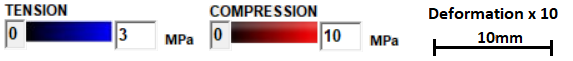
\includegraphics[width=0.8\linewidth]{Files/exp_3D/tagCS10s.png}
\end{subfigure}%


  \caption{Internal Stress in Each Step for ASR $10 \times 10 \times 10$ mm Case ($Deformation \times 10$)}
  \label{fig:ASR_Small_ASR_IS}
  \end{figure}


Also, the Inner Stress condition for each step is collected and shown in Figure \ref{fig:ASR_Small_ASR_IS}, which can also reveal many details in the expanding procedure.

From step 1 compressive stress is generated in and one layer around the reactive aggregate, due to the initial strain added to the reactive interfaces. While other paste elements located around reactive aggregate reacted in tension status.

This very small size simple example shows logically our method of adding initial strain to generate ASR expansion should work in the way we assumed.
